\documentclass[12pt]{article}
\usepackage{geometry} % see geometry.pdf on how to lay out the page. There's lots.
\geometry{a4paper} % or letter or a5paper or ... etc
\usepackage{graphicx}

% \geometry{landscape} % rotated page geometry

% See the ``Article customise'' template for come common customisations

\title{\SSEnext Modular Device Support}
\author{Dave Astels}

\def\SSEnext{SSE\kern-.1em\lower.5ex\hbox{\footnotesize next}\kern+.2ex}

%%% BEGIN DOCUMENT
\begin{document}

\maketitle
%\tableofcontents

\section{Overview}

One of the key features of the \SSEnext architecture is modular device
support. This will allow new devices to be added without having to
modify, rebuild, redownload, or reinstall \SSEnext\footnote{In the
  majority of cases. There may be new devices that require changes to
  the core apps.}.

There are three aspects of device support that we need to be concerned
with:
\begin{enumerate}
\item client,
\item database,
\item and device firmware interaction.
\end{enumerate}

Figure~\ref{fig:blockdiagram} shows the relationship between \SSEnext
and a device module.

\begin{figure}[htbp] %  figure placement: here, top, bottom, or page
   \centering
   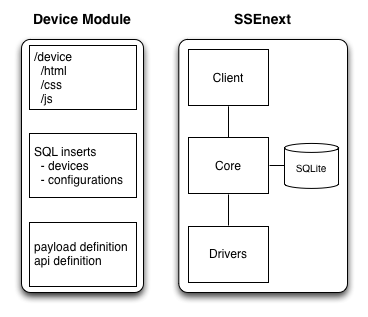
\includegraphics[width=5in]{block_diagram.png} 
\caption{Overview of modular device support.}
\label{fig:blockdiagram}
\end{figure}


This document will explore all three in order.


\section{Client}



\section{Database}

\subsection{Device record}

There needs to be a record in the \verb|records| table for each device
supported by the system.

\subsection{Configuration records}

Depending on the device, SteelSeries may create and include
configurations that are installed as part of the support of that
device. The need to be added to the \verb|configurations| table.



\section{Device interaction}



\subsection{Data definition}
\label{sec:datadefinition}

Each structure defines a conceptually complete chunk of data that
corresponds to what the firmware deals with.  Structures are created
by the \verb|def-struct| function. The first argument to
\verb|def-struct| is the name of the structure as a raw symbol (i.e.
unquoted). \verb|def-struct| can take a number of parameters which
define the fields of the structure.

Each field is defined by \verb|def-field| which takes name and type
(both as raw symbols). The name is an arbitrary symbol (with the
cavaet that it must match the corresponding name in the json used by
\SSEnext. The type must be one of \verb|uint8|, \verb|uint16|,
\verb|uint32|, or the name of another structure. In this example,
that's \verb|led|.

\begin{verbatim}
(def-struct led
     (def-field red uint8)
     (def-field green uint8)
     (def-field blue uint8)
     (def-field mode uint8))

(def-struct cpi
     (def-field unbind uint8)
     (def-field x uint16)
     (def-field y uint16)
     (def-field led led))
\end{verbatim}

These delarations are executed and result in the structure shown in
Figure~\ref{fig:defstructure}. Notice that the individual structures
are separate with inter-structure links being used to denote the
nesting. Note that these structures can be references by any number of
other structures, as well as arrays (more details on this later).

\begin{figure}[htbp] %  figure placement: here, top, bottom, or page
   \centering
   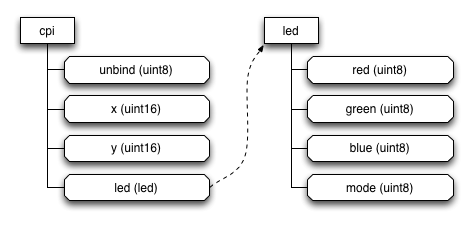
\includegraphics[width=5in]{def_structure.png} 
\caption{Definition structure.}
\label{fig:defstructure}
\end{figure}

That structure then gets processed, flattening it, tagging each field
with it's path in the original structure, and computing the bytearray
offset of each field (to ensure proper alignment). The result is shown
in Figure~\ref{fig:flattened}. Each flattened field also contains the
size of the declared type, and a link to the field node in the
original structure. Note that fields are always ordered by how they
appear in the final bytearray. The order specified in the initial
declaration code carries through to the bytearray.

\begin{figure}[htbp] %  figure placement: here, top, bottom, or page
   \centering
   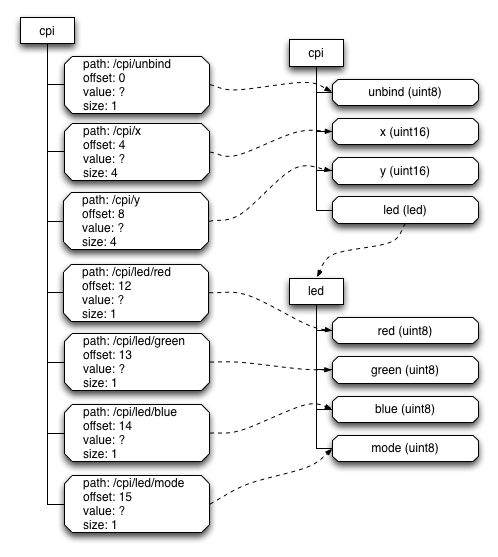
\includegraphics[height=6in]{flat_structure.png} 
\caption{processed structure.}
\label{fig:flattened}
\end{figure}

Notice that each field in the flattened structure contains a value
that is either \verb|uint8|, \verb|uint16|, or \verb|uint32|..
This will initially be 0, and will be filled in later based on either json
from \SSEnext, or bytearray data from the device.

This flattened structure provides a bridge between structured data
containing field values, as json, and the byte array required for
communication with the hardware device. Figure~\ref{fig:bytearray}
shows the bytearray that this structure corresponds to.

\begin{figure}[htbp] %  figure placement: here, top, bottom, or page
   \centering
   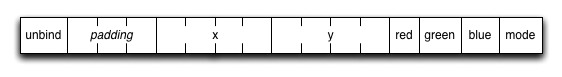
\includegraphics[width=6in]{bytearray.png} 
\caption{The bytearray}
\label{fig:bytearray}
\end{figure}

Fields within a data declaration can be arrayed. When the structure
gets processed/flattened multiple copies of these fields will be
placed in the result. To do this you provide a third arument that
specifies a repeat count. As an example, here's a declaration that
contains once simple repeated field and one complex repeated field
(see the previous structure declaration at the beginning of \S~\ref{sec:datadefinition}).

\begin{verbatim}
  (def-struct sensor
     (def-field a uint8 4)
     (def-field cpi cpi 2))
\end{verbatim}

Once this is processed and flattened, it corresponds to the byte array
shown in Figure~\ref{fig:repeatingbytearray}.

\begin{figure}[htbp] %  figure placement: here, top, bottom, or page
   \centering
   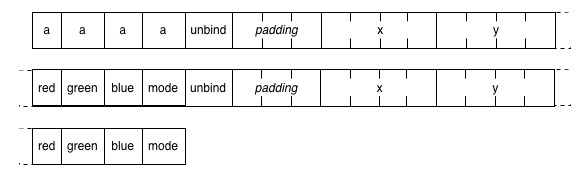
\includegraphics[width=6in]{repeated_bytearray.png} 
\caption{Bytearray with repeating fields}
\label{fig:repeatingbytearray}
\end{figure}

Now that we've covered the data interaction with the device firmware,
let us turn to the communication to the \SSEnext application. \SSEnext
deals in json, specifically json that parallel to the structure we've
declared. Going back to the structure declaration at the beginning of
\S~\ref{sec:datadefinition}, we will want json of the form:

\begin{verbatim}
{
  "cpi": {
    "unbind": 1,
    "x": 1200,
    "y": 1400,
    "led": {
      "red": 255,
      "green": 255,
      "blue": 100,
      "mode": 2
    }
  }
}
\end{verbatim}

When using json to populate the values in the fields, the paths from
the fields are used to traverse the json to find the corresponding
values. Once values are in the fields, the flattened structure can be
used to generate the bytearray. 

Conversely, the data in a bytearray can be extracted based on the
offsets and sizes in the fields and used to set the values in the
fields. Once the field values are populated, the corresponding paths
can be used to build an appropriate json structure that can be sent to
\SSEnext. 

\subsection{JSON transformations}

In the last section we went over how to declare fields, providing a
name, type, and optionally a repeat count. You can provide an
additional pair of arguments that will effect the consumption and
generation of json from the field. Note that the repeat count is still
optional. If the third arguemnt (if any) is a number, it's assumed
that you are providing a repeat count.

These two arguments are Lisp functions that are used to transform the
niave conversion to/from json. They can be either the name of a Lisp
function or a lambda expression. This function can take either one or
two arguments. The first is always the value from the json
corresponding to the field. The second is the containing structure.
The function returns nothing but can modify or replace the
corresponding value value in the json. The first is used when
generating json from the field. The second is used on the json value
before it is used to set the value of the field.

\subsection{API definition}


\end{document}
